\chapter{KHẢO SÁT TÍNH ỔN ĐỊNH CỦA HỆ THỐNG}
    Ta có hàm truyền đã tìm được ở trên là:
    \[
        G(s) = \frac{4.85}{s^2 + 53.51}
    \]
    Hệ vòng kín với phản hồi là: 
    \[
        T(s) = \frac{G(s)}{1+G(s)} 
    \]
    Phương trình đặc tính:
    \begin{align*}
        &1 + G(s) = 0 \\
        &\Leftrightarrow 1 + \frac{4.85}{s^2 + 53.51} = 0 \\
        &\Leftrightarrow s^2 + 58.36 = 0
    \end{align*}
    $\Leftarrow$ Hệ không ổn định do hệ số của $s^1$ là 0. 
    \section{Biểu đồ Bode}
    \[
        G(s) = \frac{4.85}{s^2 + 53.51}
    \]
    Phân tích:
    \begin{itemize}
        \item 1 khâu khuếch đại: K = 4.85.
        \item 1 khâu dao động bậc 2.
    \end{itemize}
    Tần số cộng hưởng: 
    \[
        \omega_n = \sqrt{53.51} = 7.315 (rad/s)
    \]
    Đặc tính tần số:
    \[
        G_1(j\omega) = \frac{4.85}{-\omega^2 + 53.51}
    \]
    \textbf{Biên độ:}
    \[
        M(\omega) = \abs{G(j\omega)} = \frac{4.85}{\abs{-\omega^2 + 53.51}}
    \]
    \[
        \Rightarrow L(\omega) = 20log(M(\omega)) = 20log(4.85) - 20log(\abs{-\omega^2 + 53.51})
    \]
    \begin{itemize}
        \item Khi $0<\omega<7.315$: biên độ tăng từ -20.85dB đến $+\infty$
        \item Với $\omega > 7.315$: 
    \end{itemize}
    \begin{align*}
        &20log(4.85) - 20log(\abs{-\omega^2 + 53.51}) \approx 20log(4.85) - 20log(\omega^2) \\
        &= 20log(4.85) - 40log(\omega) \\
        &\Rightarrow \text{Độ dốc giảm: } -40dB/decade \\
        &\Rightarrow \text{Với } \omega > 7.315: \text{ biên độ giảm từ } +\infty \text{ về } -\infty
    \end{align*}
    \textbf{Pha:}
    \begin{itemize}
        \item $\omega < 7.314$: $-\omega^2 + 53.509 > 0$, pha $\angle G_1(j\omega) = 0^\circ$,
        \item $\omega = 7.314$: $-\omega^2 + 53.509 = 0$, pha nhảy từ $0^\circ$ xuống $-180^\circ$,
        \item $\omega > 7.314$: $-\omega^2 + 53.509 < 0$, pha $\angle G_1(j\omega) = -180^\circ$.
    \end{itemize}
    \textbf{Tính độ dự trữ biên độ (GM):}
    \begin{itemize}
        \item \textbf{Tìm tần số cắt pha} ($\omega_{pc}$): Đây là tần số mà pha đạt $-180^\circ$.
        \begin{itemize}
            \item Từ phân tích pha, $\angle G_1(j\omega) = -180^\circ$ khi $\omega \geq 7.314$.
            \item Vậy $\omega_{pc} = 7.314$ rad/s.
        \end{itemize}
        \item \textbf{Tính biên độ tại $\omega_{pc}$:}
            \[
            |G_1(j\omega_{pc})| = \left| \frac{4.848}{-(7.314)^2 + 53.509} \right| = \frac{4.848}{0} \to \infty
            \]
            \[
            |G_1(j\omega_{pc})|_{dB} \to +\infty \text{ dB}
            \]
            
            \item \textbf{Độ dự trữ biên độ:}
            \[
            \text{GM (dB)} = -20 \log_{10} |G_1(j\omega_{pc})| \to -\infty \text{ dB}
            \]
        \end{itemize}
\textbf{Tính độ dự trữ pha ($\phi_M$):}           
            \begin{itemize}
                \item \textbf{Tìm tần số cắt biên độ} ($\omega_{gc}$): Đây là tần số mà $|G_1(j\omega)| = 1$ (0 dB).
                \begin{itemize}
                    \item Đặt $|G_1(j\omega)| = 1$:
                    \[
                    \left| \frac{4.848}{-\omega^2 + 53.509} \right| = 1
                    \]
                    \item Khi $\omega < 7.314$, $|-\omega^2 + 53.509| = 53.509 - \omega^2$, nên:
                    \[
                    \frac{4.848}{53.509 - \omega^2} = 1 \Rightarrow 53.509 - \omega^2 = 4.848 \Rightarrow \omega^2 = 53.509 - 4.848 = 48.661
                    \Rightarrow \omega_{gc} \approx \sqrt{48.661} \approx 6.976 \, \text{rad/s}
                    \]
                \end{itemize}
                
                \item \textbf{Tính pha tại $\omega_{gc}$:}
                \begin{itemize}
                    \item Tại $\omega_{gc} = 6.976 < 7.314$, pha $\angle G_1(j\omega_{gc}) = 0^\circ$.
                \end{itemize}
                
                \item \textbf{Độ dự trữ pha:}
                \[
                \phi_M = 180^\circ + \angle G_1(j\omega_{gc}) = 180^\circ + 0^\circ = 180^\circ
                \]
            \end{itemize}
        
    \begin{figure}[H]
        \centering
        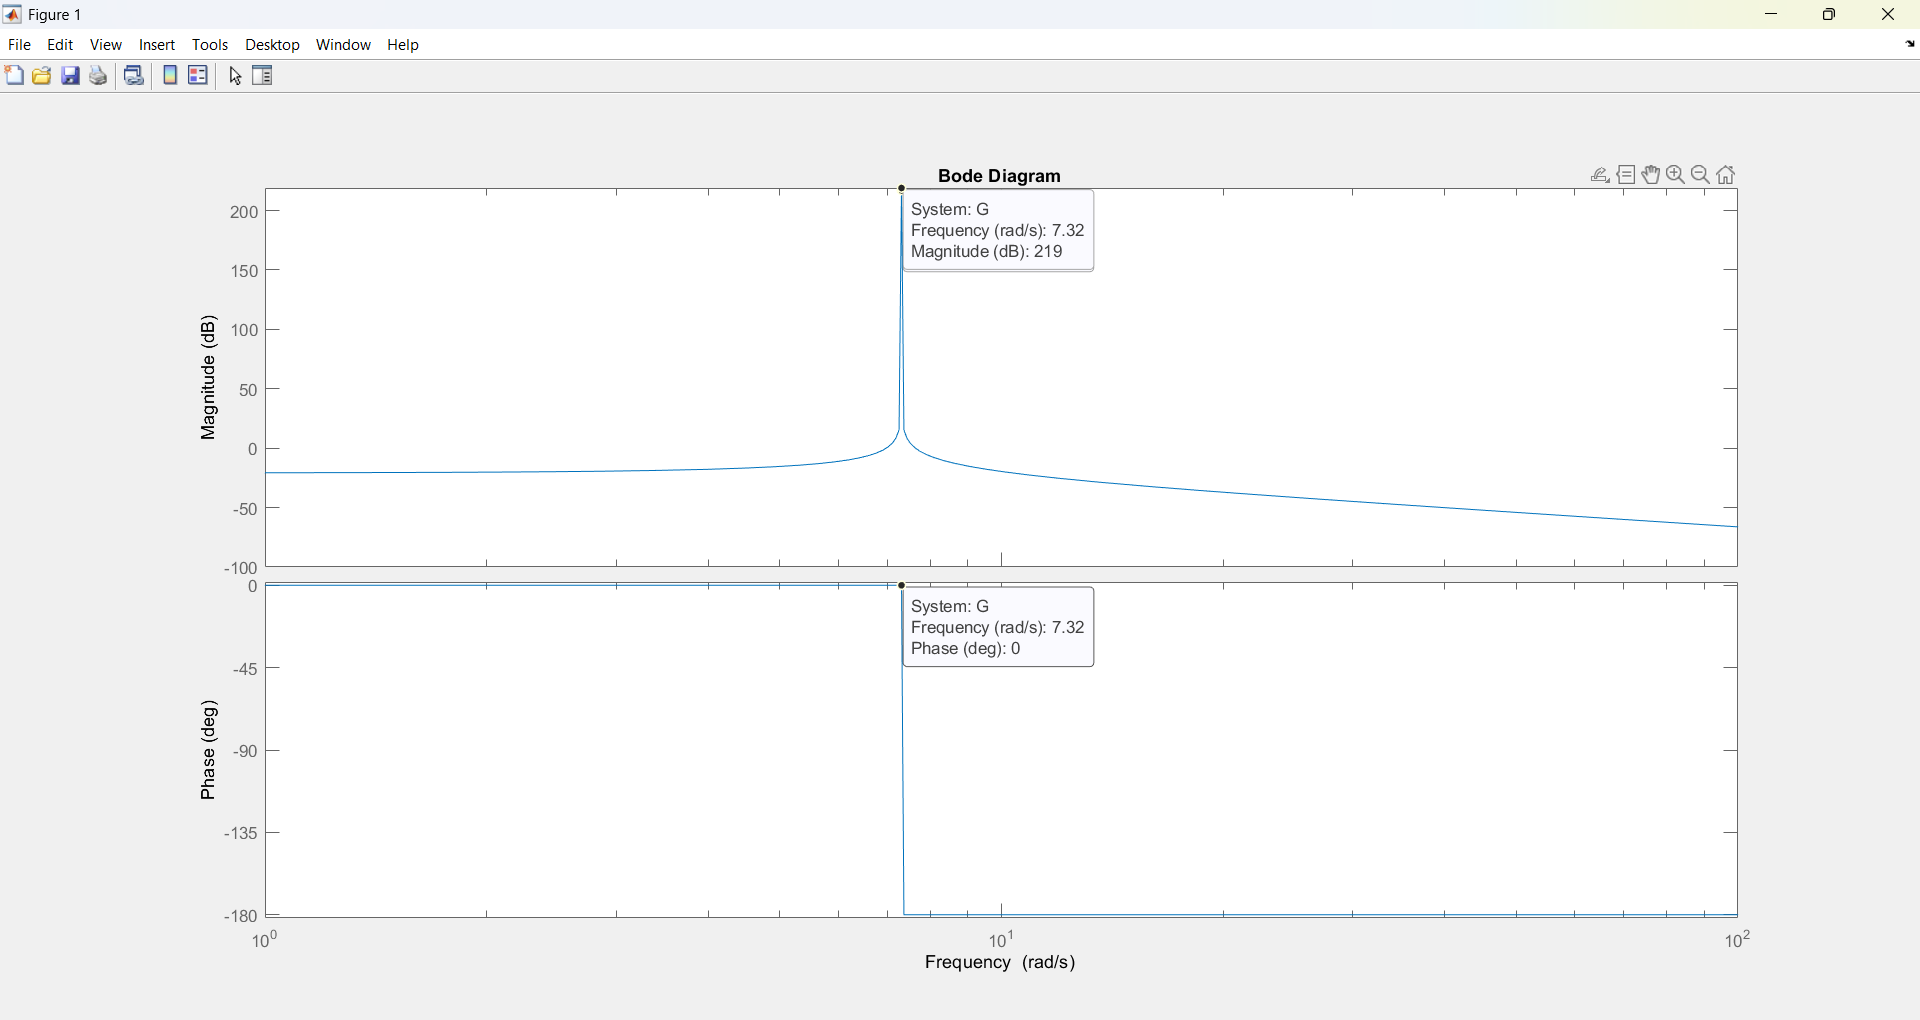
\includegraphics[width=1\textwidth]{pictures/bode.png}
    \end{figure}
    Nhận xét:
    \begin{itemize}
        \item Hệ thống vòng hở: G(s) có các cực trên trục ảo $s=+-7.315$ nên hệ thống ổn định biên. Đồ thị Bode cho thấy biên độ đạt đỉnh tại $\omega=7.315$ và pha nhảy xuống là $-180^\circ$. Điều này xác nhận hệ thống dao động không suy giảm.
        \item Từ độ thị ta có thể thấy độ dữ trữ pha $G_M < 0 dB$ nên đã vi phạm tiêu chuẩn ổn định của biểu đồ Bode $\Rightarrow$ Hệ chưa ổn định. 
    \end{itemize}
